\section{Alvan Alvanzah/1174077}
\subsection{BUKU}
Rp. 0 (Belum Lunas)

\subsection{SEJARAH PTOLEMY}
\begin{itemize}
    \item Peta
    
Peta merupakan penggambaran secara grafis atau bentuk skala (perbandingan) pada konsep mengenai bumi dalam hal ini peta merupakan alat untuk menyampaikan atau menginformasikan mengenai ilmu kebumian.
    \item Peta Menurut Claudius Ptolemaeus Ptolemy
    
Cladius Ptolemaeus yang dikenal dengan nama Ptolemy, hidup antara tahun 100 masehi dan 168 masehi, beliau merupakan salah satu sarjana sains pada masanya. Ptolemy membawa semua pengetahuan dan keterampilan matematika dan astronomi dan menerapkanya pada pembuatan peta. Data-data tentang pembuatan peta sempat hilang ketika perpustakaan Alexandria yang terkenal dibakar oleh orang-orang Kristen fanatik pada tahun 390 masehi-sebuah contoh awal konflik antara iman dan sains.
    \item Peta Dunia Ptolemy
    
Peta dunia Ptolemy adalah peta dunia yang diketahui masyarakat barat pada waktu kurun kedua masehi. Peta tersebut berdasarkan penerangan yang terkandung di dalam buku geographia, ditulis kira-kira pada 150 masehi walaupun peta autentik tidak dijumpai, buku geographia yang berisi beribu-ribu rujukan dari berbagai tempat di dunia, beserta koordinat, yang membolehkan para pelukis peta menyusun semula peta dunia Ptolemy apabila manuskripnya telah ditemui sekitar 1300 masehi.
    \item Sejarah Ptolemy

Clauduis Ptolemy adalah seorang ahli geografi, astronom, dan astrolog yang hidup pada zaman Helenistik di provinsi Romawi, Aegyptus. Claudius merupakan nomen atau nama keluarga seorang Roma, Ptolemaeus menyandang nama itu, sehingga menjadi bukti bahwa dia adalah seorang warga negara roma. Ptolemaeus (Ptolemy) adalah sebuah nama Yunani. Muncul satu kali di mitologi Yunani, dalam bentuk Homeric. Selain itu dianggap juga sebagai seorang anggota masyarakat Yunani alexandria, dan hanya sedikit yang mengetahui rincian hidup Ptolemaeus. Karya utama Ptolemy lainnya adalah Geografinya (juga disebut Geographia), kompilasi koordinat geografis dari bagian dunia yang dikenal oleh kekaisaran Romawi pada masanya.
    \item The Geography
    
Bagian pertama dari Geografi adalah diskusi tentang data dan metode yang digunakan. Seperti  model tata surya di Almagest, Ptolemy memasukkan semua informasi ini ke dalam skema besar. Ptolemaeus juga merancang dan memberikan petunjuk bagaimana membuat peta di seluruh dunia yang berpenghuni dan berprovinsi Romawi. Peta di manuskrip yang masih ada di Ptolemy’s Geography, bagaimanapun, hanya bersal dari sekitar tahun 1300, setelah teks tersebut ditemukan kembali oleh Maximus Planudes. Peta berdasarkan prinsip ilmiah telah dibuat sejak zaman Eratosthenes, pada abad ke-3 sebelum masehi, namun Ptolemy memperbaiki proyeksi peta. Karena Ptolemy berasal dari garis lintang utamanya dari nilai terpanjang minyak mentah, garis lintangnya rata-rata keliru kira-kira satu derajat, meskipun para astronom kuno mampu mengetahui garis lintang mereka lebih lama.
\end{itemize}

\subsection{Link Video}
Link Video : \texttt{https://youtu.be/TBVqN9eWO8g}

\subsection{Plagiarisme}
\begin{figure}[!htbp]
\centering
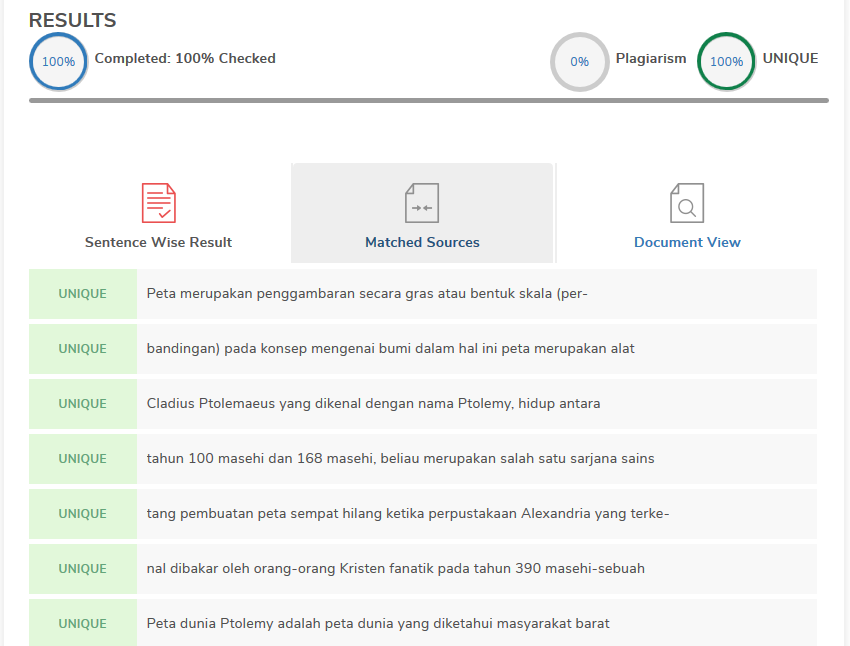
\includegraphics[width=12cm,height=8cm]{figures/tugas1/1174077/plagarisme.PNG}
\caption{Hasil Plagiarisme}
\label{penanda}
\end{figure}